\begin{frame}
    \frametitle{Planning transfer}
    \begin{block}{}
        We finally achieved a stable low earth orbit. We need to plan our transfer to our target body
    \end{block}
\end{frame}
\begin{frame}
    \begin{center}
        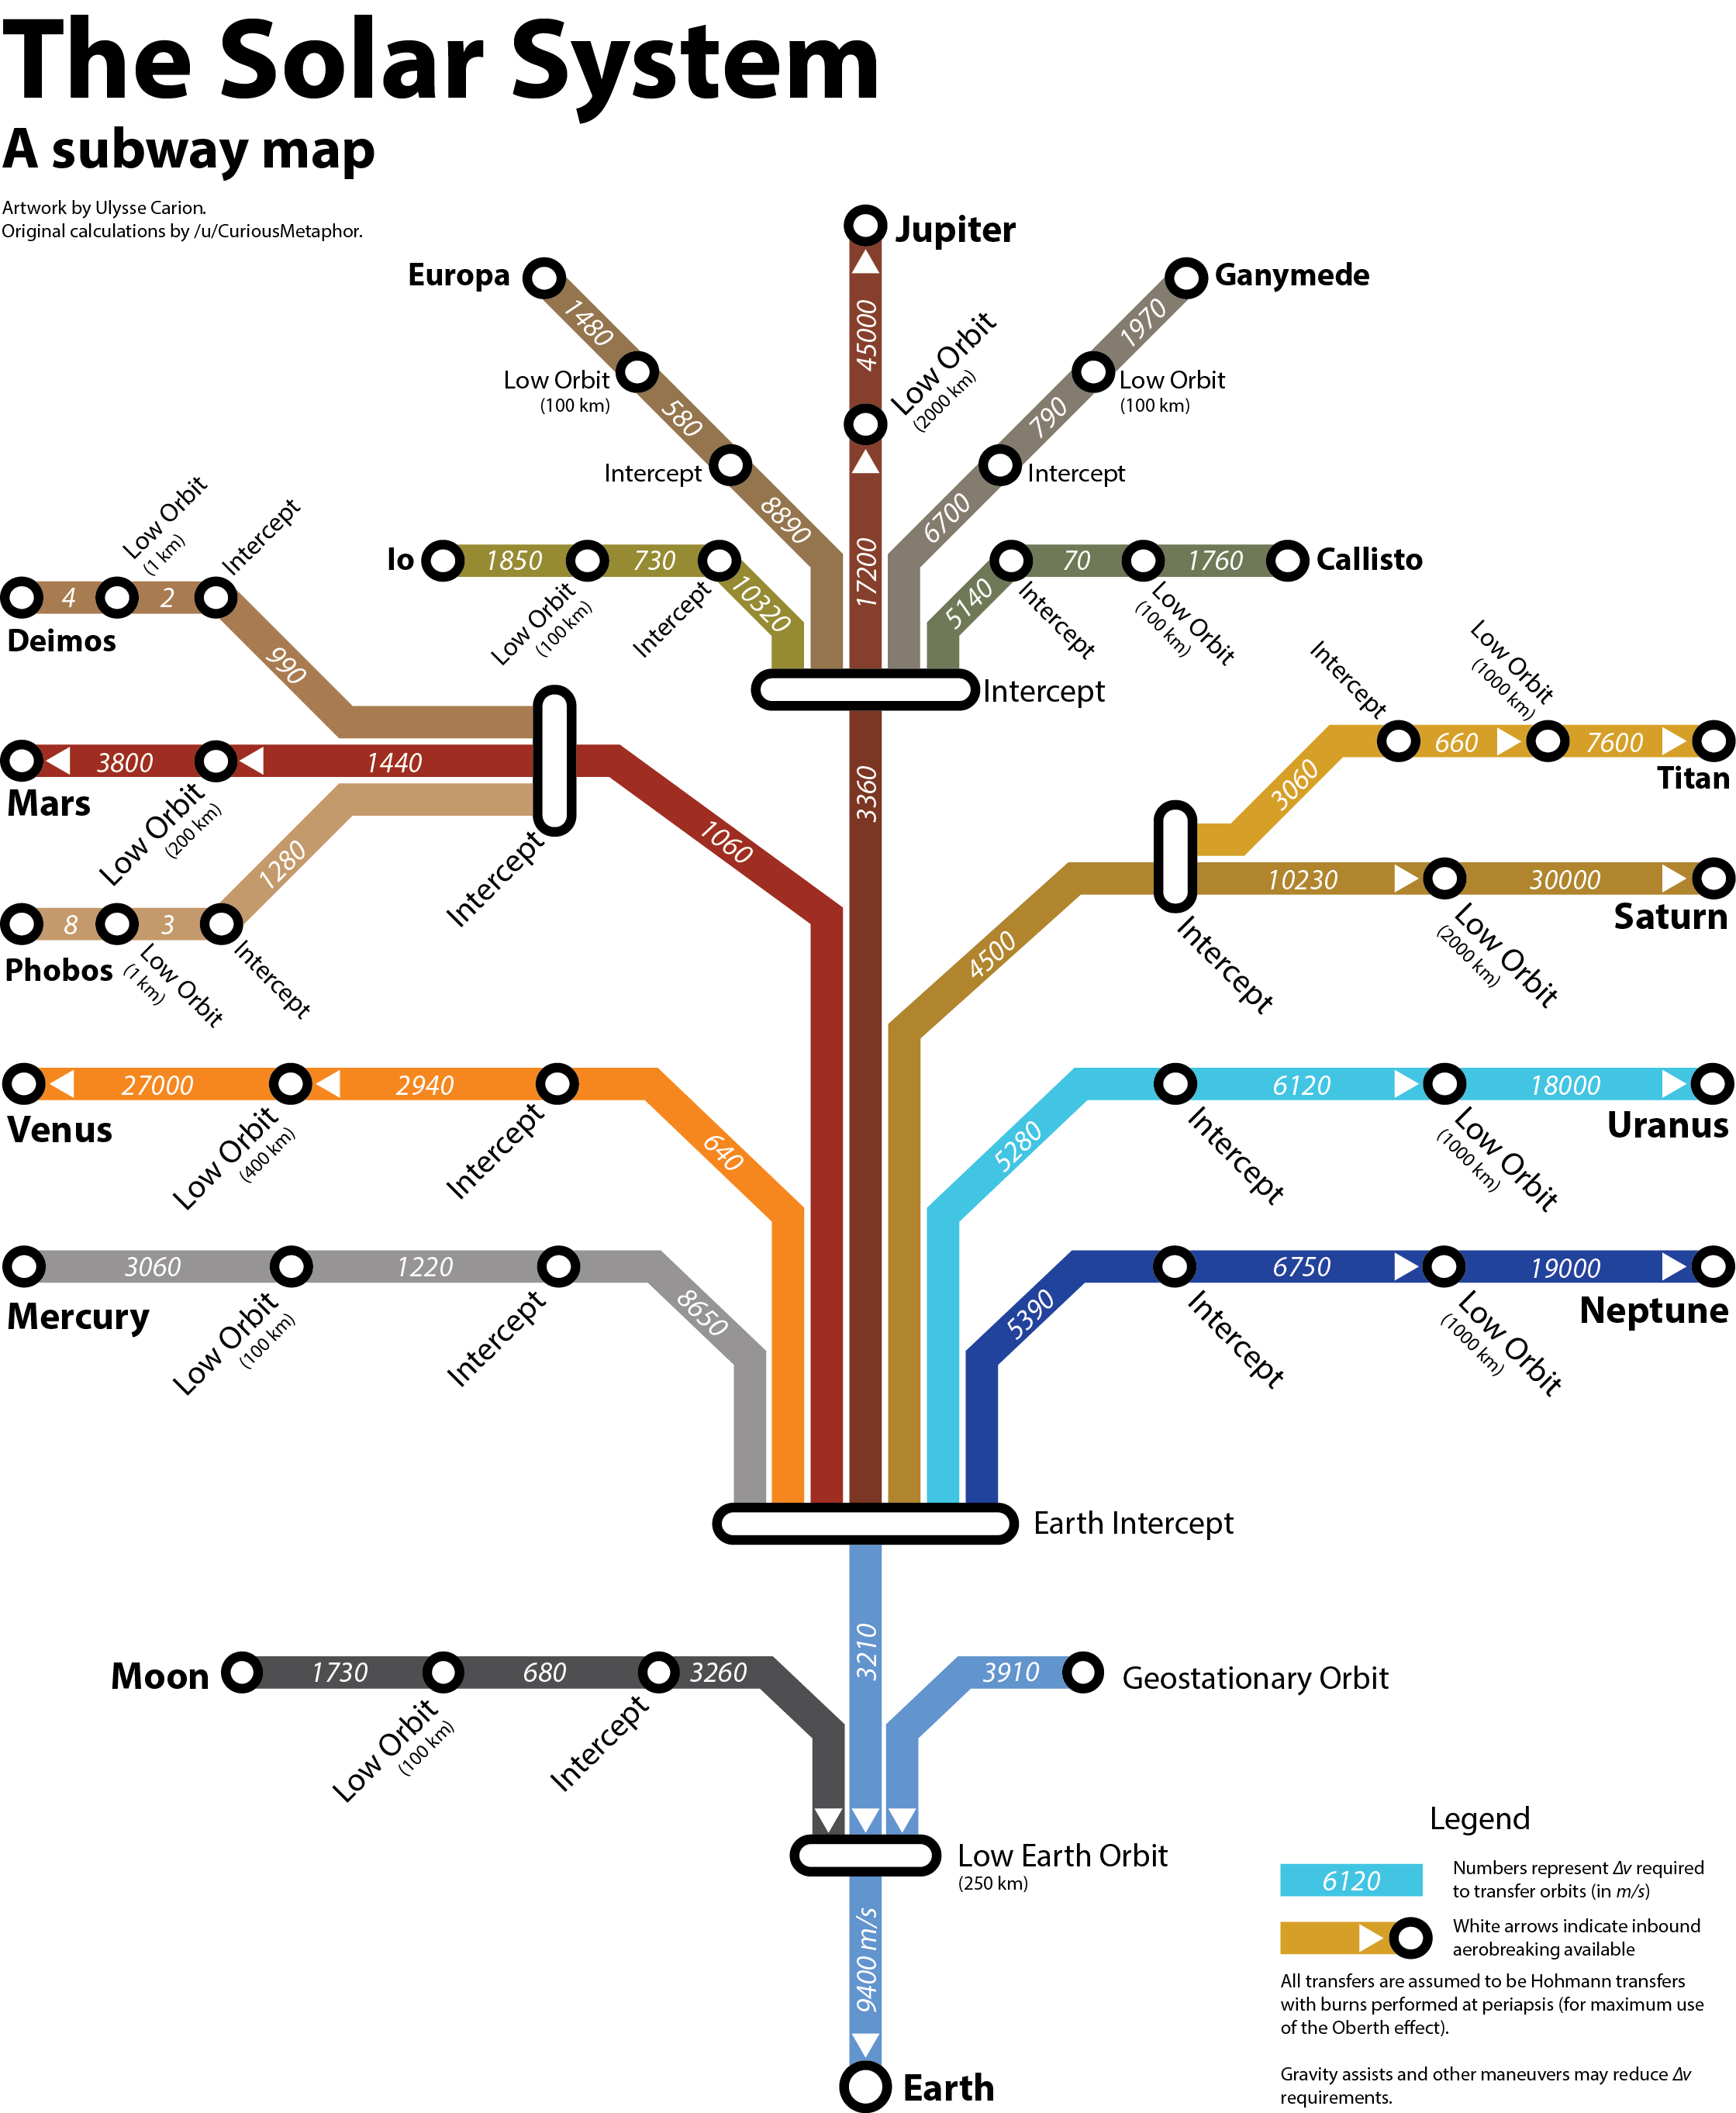
\includegraphics[height=\textheight]{images/deltavmap}
    \end{center}
\end{frame}
\begin{frame}
    \frametitle{Hohmann transfer}
    \begin{block}{}
        Now that we know our target and know the delta-v required to get there we need to plan the encounter
    \end{block}
    \begin{block}{}
        \begin{center}
            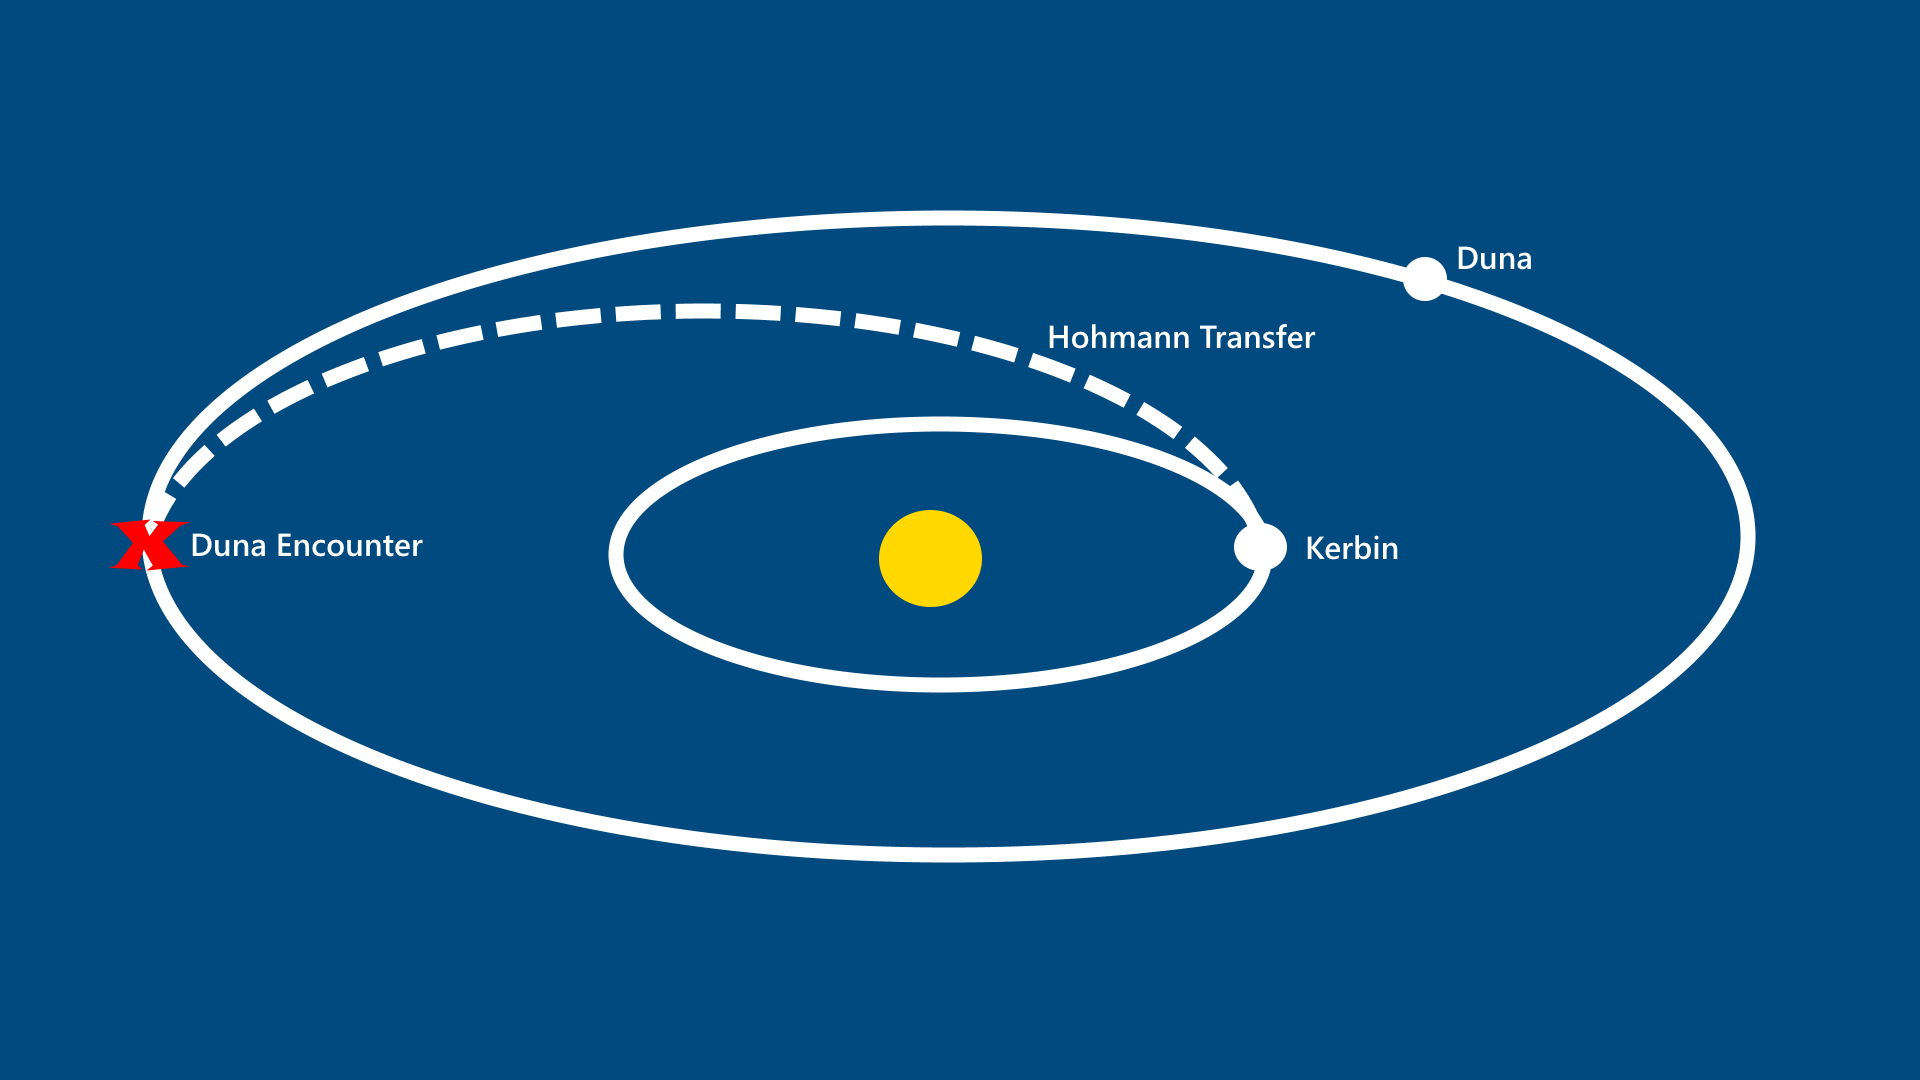
\includegraphics[scale=0.2]{images/hohmann_transfer}
        \end{center}
    \end{block}
\end{frame}
\begin{frame}
    \frametitle{Hohmann transfer window}
    \begin{block}{}
        To be able to transfer with the least amount of delta-v possible, we need to launch when the target body is
        at an optimal position
    \end{block}
    \begin{block}{}
        \begin{center}
            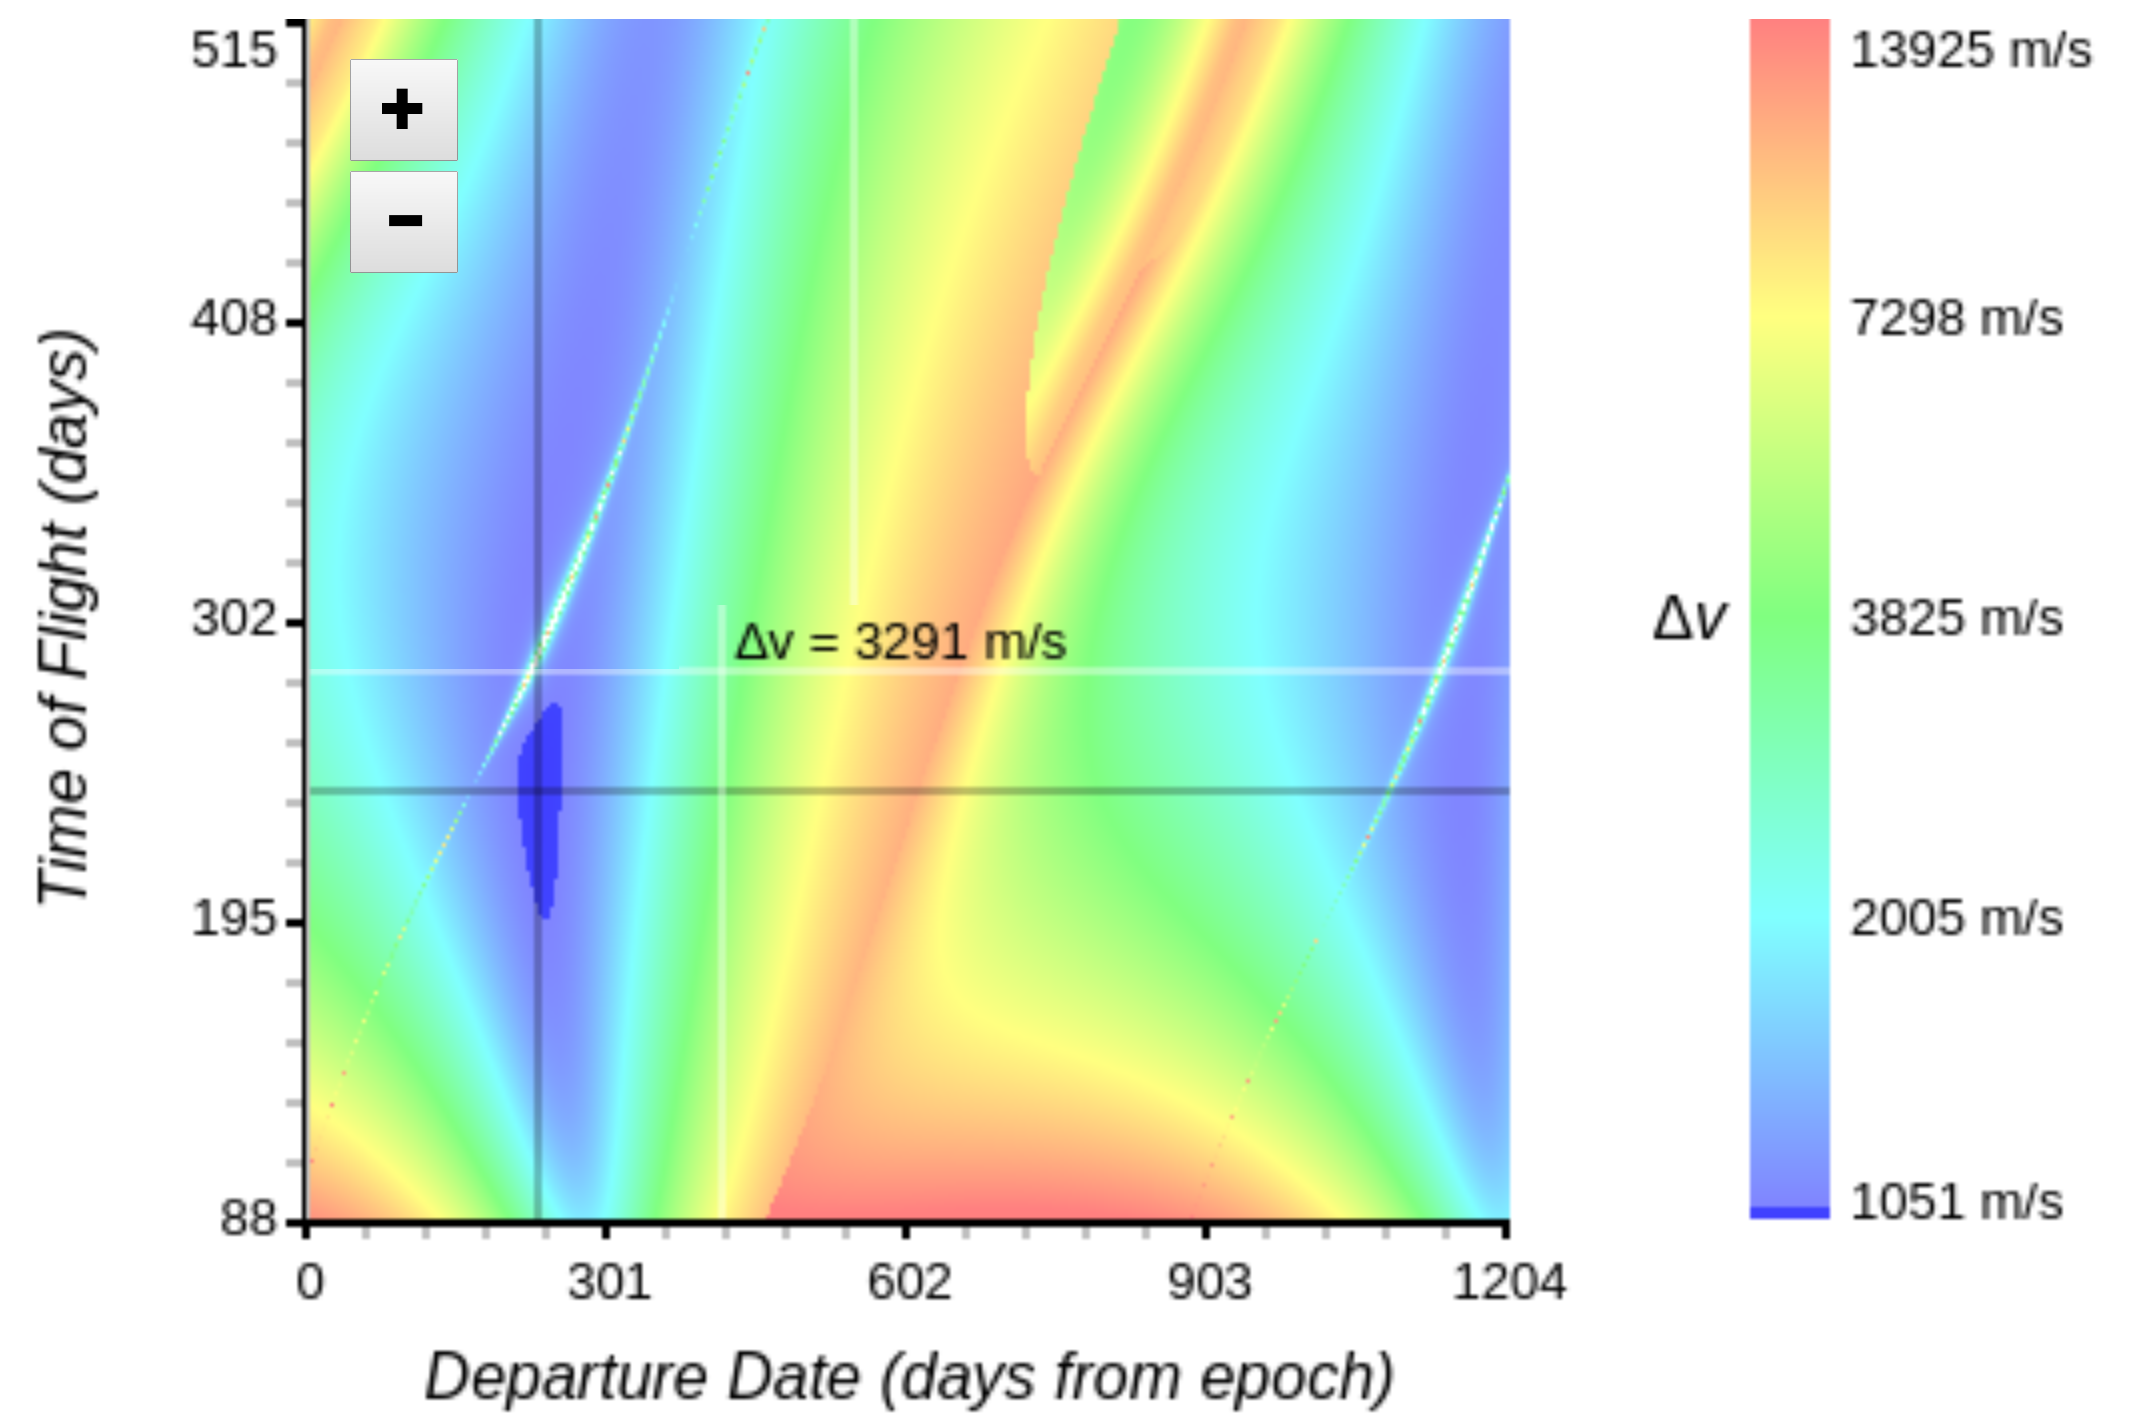
\includegraphics[scale=0.08]{images/hohmann_transfer_window}
        \end{center}
    \end{block}
\end{frame}
{
\usebackgroundtemplate{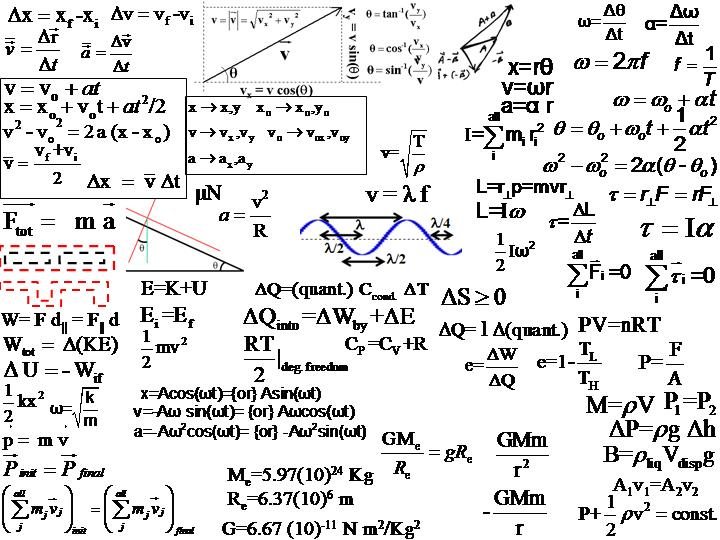
\includegraphics[width=\paperwidth]{images/oberth_troll}}%
\begin{frame}[t]{Oberth effect}
\end{frame}
}
\begin{frame}[t]{jk, Oberth effect}
    \begin{block}{}
        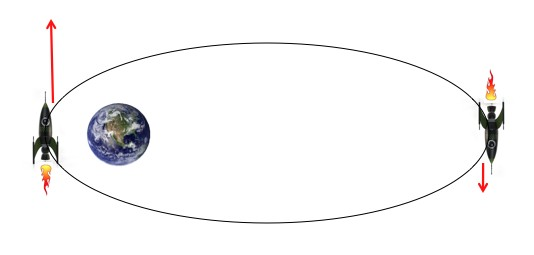
\includegraphics[width=\textwidth]{images/obert_effect}
    \end{block}
\end{frame}
\begin{frame}[t]{Escape}
    \begin{block}{}
        With the Oberth effect we can begin our escape burn and start our transfer orbit
    \end{block}
    \begin{block}{}
        \begin{itemize}
            \item Decelarate to drop orbit deeper into the gravity well
            \item Wait for lowest point of orbit (to make maximal use of Oberth effect)
            \item Make transfer burn and coast to encounter
        \end{itemize}
    \end{block}
\end{frame}
